\documentclass[10pt]{article}

\usepackage[document]{ragged2e}

% for pdflatex
\usepackage[utf8]{inputenc}
% for hyperlink
\usepackage{hyperref}
\hypersetup{
    colorlinks=true,
    linkcolor=blue,
    filecolor=magenta,
    urlcolor=cyan,
}
% for table spanning multiples pages
\usepackage{longtable}
% for custom enum
\usepackage{enumitem}
% for removing alinea begin of paragraph
\usepackage{parskip}
\usepackage{array, xcolor, graphicx}
\usepackage[a4paper, margin=1cm]{geometry}
\title{\bfseries{\huge{Ingénieur Blockchain \& Data Science}}\\[0.75cm] \Large{4 années d'expérience dans la blockchain et les cryptomonnaies} }
% no author
\author{\bfseries\Huge \vspace{-4ex}}
% no date
\date{}
% custom for column style
\definecolor{lightgray}{gray}{0.8}
% custom for column type
\newcolumntype{L}{p{0.2\textwidth}}
% custom for column type
\newcolumntype{R}{p{0.75\textwidth}}
% custom for column type
\newcommand\VRule{\color{lightgray}\vrule width 2pt}
% for bullet point outside of list
\newcommand{\tabitem}{~~\llap{$\rightarrow$}~~}
\begin{document}

\begin{minipage}[t]{0.80\textwidth}
\textbf{\Large{Mohamed Amine LEGHERABA}}\\
\vspace{4ex}26 ans\\
92 bis rue Rouget de Lisle, Bezons, France\\
\href{tel:0630829000}{06 30 82 90 00}\\
\href{mailto:mlegheraba@protonmail.com}{mlegheraba@protonmail.com}\\
\href{https://github.com/MohamedLEGH}{github.com/MohamedLEGH}\\
\vspace{5ex}{\bf Français}: langue maternelle \\
{\bf Anglais}: bon niveau (TOIEC: 935) \\
\end{minipage}
\begin{minipage}[t]{0.20\textwidth}
\vspace{-3ex}
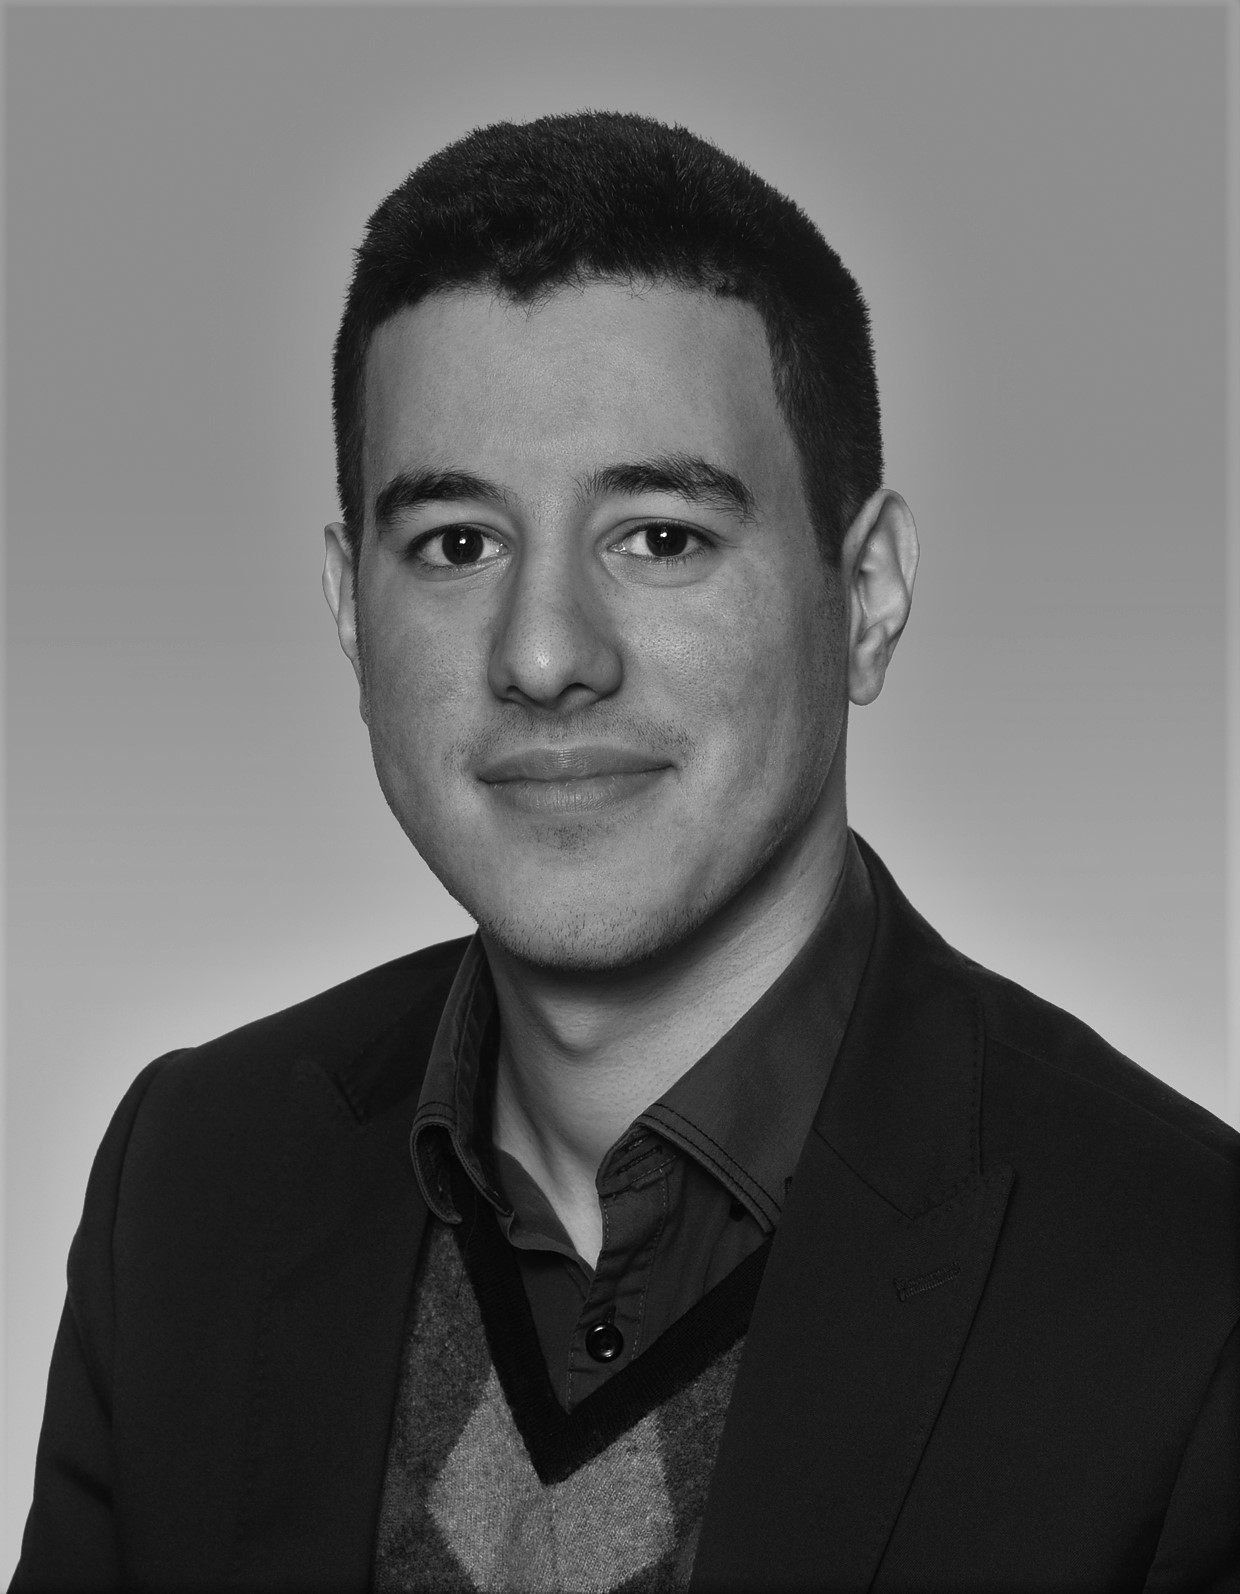
\includegraphics[width=4cm]{figures/Legheraba-Mohamed-White.jpg}
\end{minipage}
% to make maketitle work without begin of page
{\let\newpage\relax\maketitle}
% to remove page number
\thispagestyle{empty}

\vspace{-10ex}

\section*{Formation}

\vspace{2ex}

\begin{tabular}{L!{\VRule}R}
\textbf{\textit{2015--2018}} \hspace{1.5ex} 
\includegraphics[width=1.4cm]{figures/Logo_Reseau_Polytech.png} & \textbf{Diplôme d'Ingénieur, Polytech Sorbonne}, spécialité \textit{Mathématiques Appliquées et Informatique Numérique}: Statistiques, Équations différentielles, Programmation, Structures de données, Parallélisme.\\[0.75cm]
\textbf{\textit{2017 (Hiver)}} \hspace{.5ex} 
\includegraphics[width=.85cm]{figures/TU.png} & \textbf{Semestre Erasmus à TU Delft}, Pays-Bas: Théorie des graphes, Cryptographie, Blockchain, Cloud Computing, Visualisation de données.\\[0.75cm]
\textbf{\textit{2013--2015}} \hspace{5ex} 
\includegraphics[width=.85cm]{figures/PEIP_logo.png}  & \textbf{Polytech Sorbonne},  \textit{PeiP} (Parcours des écoles d'ingénieurs Polytech): Maths, Informatique, Physique, Chimie, Mécanique.\\[0.75cm]
\textbf{\textit{2013}} & \textbf{Baccalauréat S}, mention Bien. Lycée Chaptal. \\
\end{tabular}

\vspace{2ex}

\section*{Expérience Professionnelle}

\vspace{2ex}

\begin{longtable}{L!{\VRule}R}
\textbf{\textit{Depuis Avril 2019}}& 
\includegraphics[width=2cm]{figures/SIA_logo.png} \hspace{0.2cm} {\bf Ingénieur Blockchain \& Data Science, Sia Partners, en cours.} \\[0.25cm]

& \tabitem \small{\textbf{Experimentations MNBC à la Banque de France} (membre du pôle blockchain en tant qu'expert technique, cadrage technique d'une expérimentation, support technique pour 2 autres expérimentations, formation des autres membres de l'équipe sur la Blockchain et la méthodologie DevOps, implémentation des pipelines CI/CD)}

\\[0.20cm]
& \tabitem \small{\textbf{Suivi des limites de trading à l'aide d'un réseau blockchain pour un fonds d'investissement} (expert blockchain, implémentation d'un réseau blockchain privé, développement de smart contract et d'un système d'oracle, audit de code, supervision, mise en place de tests) \it{Mission que j'ai obtenu moi-même grâce à mon réseau et que j'ai accompli de bout en bout}}

\\[0.20cm]
& \tabitem \small{\textbf{Création d'une application de paiement mobile en cryptomonnaies pour un distributeur français} (expert blockchain, développement d'une interface de paiement sécurisée, développement de l'application de back-office et d'une solution de sécurisation des fonds de cryptomonnaies et d'échange avec des euros)}

\\[0.20cm]
& \tabitem \small{\textbf{Enregistrement du consentement du patient sur la blockchain avec des signatures numériques pour un acteur du secteur public} (dans le context des essais cliniques, implémentation d'une interface pour collecter les signatures numériques du patient et du médecin, envoie du hash des signatures sur le réseau Ethereum, interface web pour vérifier la validité de l'enregistrement)}

\\[0.20cm]
& \tabitem \small{\textbf{Certification du niveau de décibels sur le réseau Ethereum pour un opérateur de transport} (IoT \& Blockchain, réception des données du niveau de décibel via une connexion Bluetooth, transfert de l'interformation sur la blockchain quand la valeur dépasse la limite définie, affichage des valeurs en temps réel sur une interface web)}

\\[0.20cm]
& \tabitem \small{\textbf{Smart Data Quality: Application de filtrage et de visualisation des données pour aider le consultant pendant sa mission} (développement d'algorithmes de Data Science en Python, optimisation du code, déploiement sur l'infrastructure AWS, ...)}

\\[0.20cm]
& \tabitem \small{\textbf{Projet Heka: \href{https://heka.sia-partners.com/fr}{Usine logicielle} pour les applications Data Science} (développement des microservices en Python et en React, déploiement continu sur l'infrastructure Kubernetes, ...)}

\\[0.20cm]
& \tabitem \small{\textbf{Veille R\&D sur la blockchain, les cryptomonnaies et les systèmes distribués} (étude des réseaux blockchain Liquid, Libra et TON, des technologies Lightning Network, HTLC Atomic Swap, Zero-knowledge proofs, Raft protocol, Taproot et Multi-Party Computation, ...)}

\\[0.20cm]
& \tabitem \small{\textbf{Rédaction d'articles} (\href{https://www.sia-partners.com/fr/actualites-et-publications/de-nos-experts/la-blockchain-catalyseur-de-la-decentralisation-et-de-la}{\textit{Blockchain \& 5G}}, \href{https://www.sia-partners.com/fr/actualites-et-publications/de-nos-experts/entretien-avec-pierre-noizat-bitcoin-et-cryptomonnaies-0}{\textit{Interview de Pierre Noizat}}, ...)}

\\[0.20cm]
& \tabitem \small{\textbf{Enseignement \textit{Programmer une blockchain}} (\href{https://github.com/MohamedLEGH/tutoriel-blockchain-creation-bootstrap}{Polytech Sorbonne}, \href{https://github.com/MohamedLEGH/tutoriel-blockchain-MinesBootstrap}{Mines St Etienne}, ...)}

\\[0.20cm]
\textbf{\textit{Mars--Septembre 2018}}& 
\includegraphics[width=1.5cm]{figures/ofi-am.png} \hspace{0.2cm} {\bf Stagiaire veille R\&D, Département Développement, OFI AM, 6 mois}.\\
& \small{Veille autour des technologies de Blockchain, de l’automatisation de tâches avec Airflow, de la conteneurisation d’application avec Docker et de la supervision système avec Tableau Server.} \\


\\[0.20cm]
\textbf{\textit{2017}}& {\bf Développement pour plusieurs ICO, dont 2 qui ont levé plus de 5M\$}.\\
& \small{Développement de smart contracts pour la mise en place des tokens, mise en place d'un protocole de sécurité pour le stockage de cryptomonnaies, création de scripts pour intéragir avec la blockchain Ethereum.} \\


\end{longtable}

\vspace{2ex}

\section*{Compétences Techniques}

\vspace{2ex}

\begin{tabular}{ l l }
\textbf{Blockchain}: Ethereum, Corda, Hyperledger, Bitcoin & \textbf{DevOps}: Kubernetes, Gitlab CI/CD, GCP, Terraform \\[0.1cm]
\textbf{Smart contracts}: Solidity, Corda contrats, Chaincodes & \textbf{Outils}: Shell, Git, Docker, VS Code, PowerPoint \\[0.1cm]
\textbf{Mathématiques}: Cryptographie, Statistiques, Graphes & \textbf{Programmation}: Python, JavaScript, Bash, C/C++, Kotlin, R \\[0.1cm]
\textbf{Bases de données}: PostgreSQL, MySQL, SQLAlchemy & \textbf{Frameworks}: ReactJS, Node.js, Ethers.js, Flask, Web3.py, PyQt \\[0.1cm]
\textbf{Protocoles}: Lightning Network, IPFS, TCP/IP & \textbf{Méthodologie}: Méthode Agile, APIs REST, Microservices \\[0.1cm]
\end{tabular}

\vspace{2ex}

\section*{Compétences Fonctionnelles et Business}

\vspace{2ex}

\begin{tabular}{ l }
\textbf{Réseaux blockchain privées \& publiques}: différences dans le cas d'usage, choix du framework.\\[0.1cm]
\textbf{Finance décentralisée} : Stablecoins, protocoles Defi, sécurisation des clés privées, connexion avec la finance traditionnelle.\\[0.1cm]
\textbf{MNBC \& Infrastructures de Marchés}: Implications d'un crypto euro, Target2 \& Target2 Securities, PvP \& DvP.\\[0.1cm]
\textbf{Audit}: Audits de smart contracts, audits de technologies blockchain, audits de startups \& fintechs Blockchain.\\[0.1cm]
\end{tabular}

\vspace{1ex}

\section*{Contributions Associatives}

\vspace{2ex}

\begin{tabular}{L!{\VRule}R}
\textbf{\textit{Depuis 2018}} & Association \textbf{Le Trait D’Union}, Aide aux devoirs auprès de lycéens et de collégiens. Rédaction de dossiers de subventions, trésorier. \\[0.75cm]

\textbf{\textit{2014--2017}} & Association étudiante \textbf{Averroès}, Dons alimentaire pour les étudiants, trésorier puis président. \\
\end{tabular}

\vspace{2ex}

\section*{Loisirs}

\vspace{2ex}

\hspace*{1ex} \textbf{Électronique} (console retrogaming avec un Raspberry Pi, contrôle d'un ventilateur via un transistor, ...) \\
\hspace*{1ex} \textbf{Étude des doctrines socio-économiques} (libéralisme, école autrichienne d'économie, anarchisme, technoéthique, ...) \\
\end{document}
